\let\negmedspace\undefined
\let\negthickspace\undefined
\documentclass[journal,12pt,onecolumn]{IEEEtran}
\usepackage{cite}
\usepackage{amsmath,amssymb,amsfonts,amsthm}
\usepackage{algorithmic}
\usepackage{graphicx}
\usepackage{textcomp}
\usepackage{xcolor}
\usepackage{txfonts}
\usepackage{listings}
\usepackage{enumitem}
\usepackage{mathtools}
\usepackage{gensymb}
\usepackage{comment}
\usepackage[breaklinks=true]{hyperref}
\usepackage{tkz-euclide} 
\usepackage{listings}
\usepackage{gvv}                                        
\def\inputGnumericTable{}                                 
\usepackage[latin1]{inputenc}                                
\usepackage{color}                                            
\usepackage{array}                                            
\usepackage{longtable}                                       
\usepackage{calc}                                             
\usepackage{multirow}                                         
\usepackage{hhline}                                           
\usepackage{ifthen}                                           
\usepackage{lscape}

\newtheorem{theorem}{Theorem}[section]
\newtheorem{problem}{Problem}
\newtheorem{proposition}{Proposition}[section]
\newtheorem{lemma}{Lemma}[section]
\newtheorem{corollary}[theorem]{Corollary}
\newtheorem{example}{Example}[section]
\newtheorem{definition}[problem]{Definition}
\newcommand{\BEQA}{\begin{eqnarray}}
\newcommand{\EEQA}{\end{eqnarray}}
\newcommand{\define}{\stackrel{\triangle}{=}}
\theoremstyle{remark}
\newtheorem{rem}{Remark}
\usepackage{circuitikz}
\begin{document}

\bibliographystyle{IEEEtran}
\vspace{3cm}

\title{ASSIGNMENT-2}
\author{AI24BTECH11012-Pushkar Gudla}
\maketitle
\bigskip
\section*{\textbf{Vector Arithmetic(CBSE)}}

\textbf{Question:} If $\myvec{3,3}$, $\myvec{6,y}$, $\myvec{x,7}$ and $\myvec{5,6}$ are the vertices of a parallelogram taken in order, find the values of $x$ and $y$. 
		\hfill{(10, 2011)}\\

		\solution Property: midpoints of diagnol coincide. Let $\vec{O}$ be the midpoint of the diagnols.\\

		$\vec{O}=\frac{\myvec{3\\3}+\myvec{x\\7}}{2}$\\
		from here we get $\vec{O}=\myvec{(3+x)/2 \\ 5}$, we also have\\
		$\vec{O}=\frac{\myvec{6\\y}+\myvec{5\\6}}{2}$\\
		this gives us $\vec{O}=\myvec{5.5\\(y+6)/2}$\\
		On comparing the above two values of $\vec{O}$, we get the values of $x$ and $y$ as:\\
		$x=8, y=4$\\
\graphicspath{ {./figs/} }
		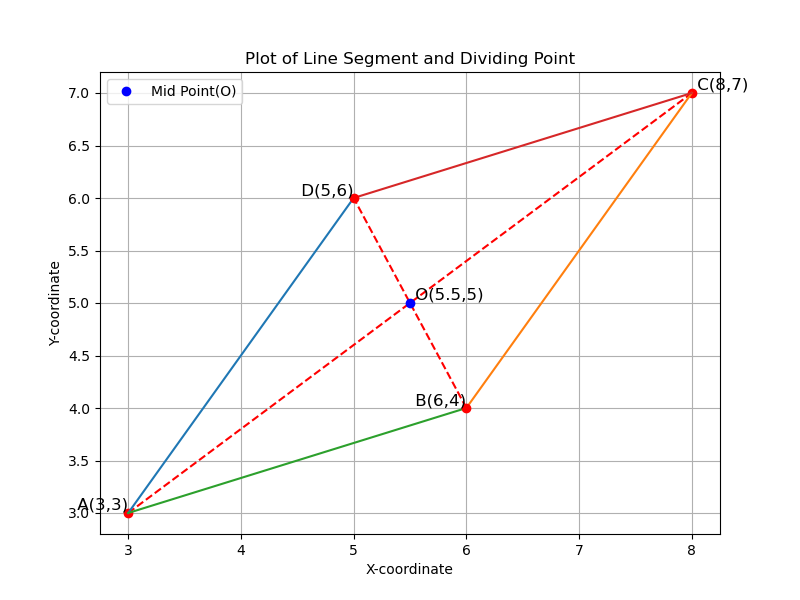
\includegraphics[scale=0.7]{parallelogram}

\end{document}
